\section{Spring and Mass System}

Let $r = \sqrt{x^2 + y^2}$ be the magnitude of the position vector, and $\hat{e} = \frac{x\mathbf{i} + y\mathbf{j}}{r}$ be the unit vector in the radial direction.

% The coupled differential equations
\begin{align}
    \ddot{x} &= -\frac{k}{m} \left( r - L_0 \right) \frac{x}{r} \label{eqn:question7_eomx}\\
    \ddot{y} &= -g - \frac{k}{m} \left( r - L_0 \right) \frac{y}{r} \label{eqn:question7_eomy}
\end{align}

\begin{minted}{julia}
# ---- Helpers ---- #
# System Parameter Structure
Base.@kwdef struct SpringSystemParameters
    m::Float64  = 1.0
    k::Float64  = 1.0
    L0::Float64 = 0.0
    g::Float64  = 0.0
end

# ---- Define System ---- #
# System Dynamics
function spring_system(u, p, t)
    x, y, vx, vy = u
    m, k, L0, g = p.m, p.k, p.L0, p.g

    # Geometry
    r = hypot(x, y)
    if r == 0.0
        e_x, e_y = 0.0, 0.0
    else
        e_x, e_y = x / r, y / r
    end

    deltaL = r - L0

    # Forces
    F_spring_mag = -k * deltaL
    F_spring_x   = F_spring_mag * e_x
    F_spring_y   = F_spring_mag * e_y

    F_grav_x = 0.0
    F_grav_y = -m * g

    F_net_x = F_spring_x + F_grav_x
    F_net_y = F_spring_y + F_grav_y

    ax = F_net_x / m
    ay = F_net_y / m

    return [vx, vy, ax, ay]
end

params = SpringSystemParameters(
    m=1.0, k=1.0,
    L0=0.0, g=0)

u0 = [1.0, 0.0, 0.0, 1.0]   # [x0, y0, vx0, vy0]
tspan = (0.0, 10.0)         # Time span

# ---- Solver ---- #
sim_name :: String = "Problem_6/figures/circular_trajectory"

# Define ODEProblem and solve with Tsit5
prob = ODEProblem(spring_system, u0, tspan, params)
sol = solve(prob, Tsit5(), saveat=1e-3)

# Extract states directly from solution object
t = sol.t
x = sol[1, :]
y = sol[2, :]
\end{minted}


\begin{itemize}
\item \textbf{No Spring (k=0):} In the absence of spring force, the mass behaves as a projectile. It falls vertically if the initial velocity is zero and follows a parabolic trajectory if the initial velocity is non-zero.
\item \textbf{Rigid Connection ($k\approx 10^5$ ):} Theoretically, an infinitely stiff spring should mimic a rigid pendulum. With the right initial conditions ($\Delta L = 0, \vec{v}_0 = 0$), this result is observed in the numerical solution.
\item \textbf{Zero Gravity and Velocity (g=0,v=0):} Under these conditions, the system's motion is constrained to a straight line, as there are no external lateral forces to perturb the radial oscillation of the spring.
\item \textbf{Zero Rest Length $(L_0 = 0)$:} When the rest length is zero, the spring force becomes perfectly linear along both the x and y axes. This simplifies the system into a 2D harmonic oscillator, causing the mass to move along a radial line passing through the origin.
\end{itemize}

\begin{figure}[htbp]
     \centering
     % --- Row 1 ---
     \begin{subfigure}[b]{0.45\textwidth}
         \centering
         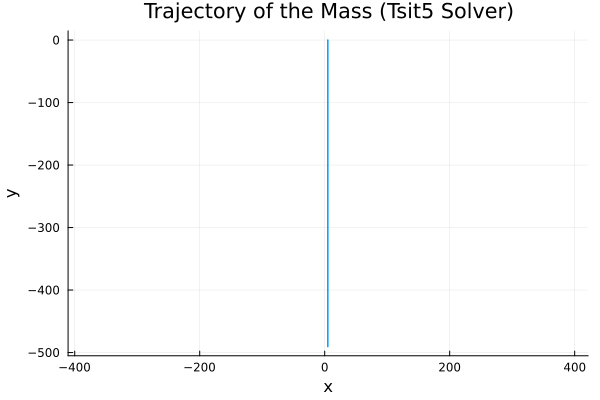
\includegraphics[width=\textwidth]{Problems/Problem6/figures/nospring_trajectory.png}
         \caption{No Spring ($k=0$)}
         \label{fig:k0}
     \end{subfigure}
     \hfill
     \begin{subfigure}[b]{0.45\textwidth}
         \centering
         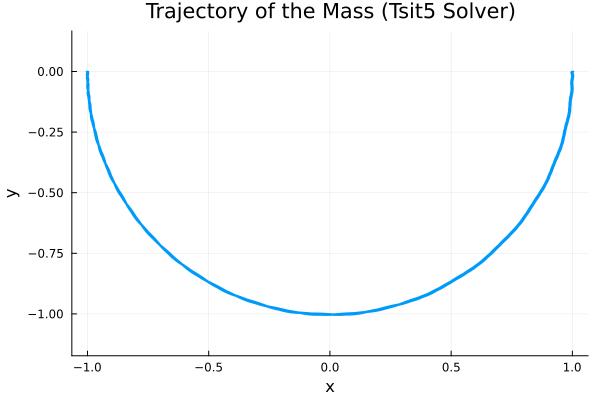
\includegraphics[width=\textwidth]{Problems/Problem6/figures/rigidspring_trajectory.png}
         \caption{Rigid Connection}
         \label{fig:rigid}
     \end{subfigure}

     \vspace{0.5cm} % Add some vertical spacing between rows

     % --- Row 2 ---
     \begin{subfigure}[b]{0.45\textwidth}
         \centering
         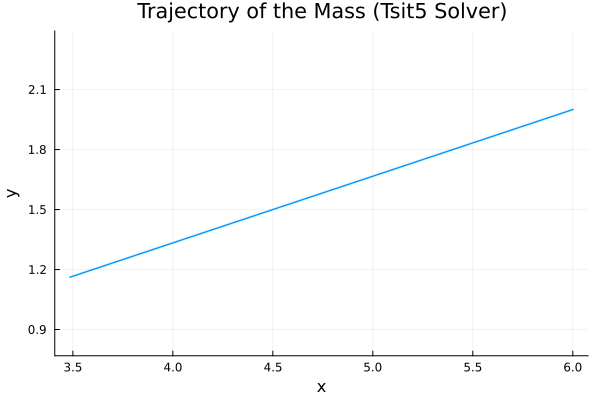
\includegraphics[width=\textwidth]{Problems/Problem6/figures/nog_trajectory.png}
         \caption{Zero Gravity ($g=0$)}
         \label{fig:g0}
     \end{subfigure}
     \hfill
     \begin{subfigure}[b]{0.45\textwidth}
         \centering
         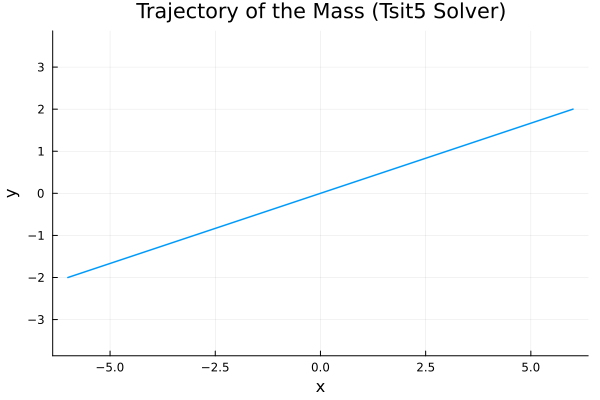
\includegraphics[width=\textwidth]{Problems/Problem6/figures/noL_harmonic_trajectory.png}
         \caption{Zero Rest Length ($L_0=0$), Harmonic Oscillator}
         \label{fig:L0}
     \end{subfigure}
     
     \caption{Numerical Simulation Results for Various System Parameters}
     \label{fig:results_grid}
\end{figure}

\subsection{A Challenge: Circular Motion in the Harmonic Oscillator}
In this subsection we attempt to derive the system parameters required to simulate circular motion in the \textbf{Zero Rest Length} case where the system behaves like a 2D harmonic oscillator.\\

Any 2D system in circular motion may be described with the positions

\begin{align}
    x &= A\cos(\omega t) \\
    y &= A\sin(\omega t).
\end{align}

which result in the second order derivatives

\begin{align}
    \ddot{x} &= -A\omega^2\cos(\omega t) \\
    \ddot{y} & = -A\omega^2\sin(\omega t).
\end{align}

Applying these solutions to Eq. \eqref{eqn:question7_eomx} and Eq. \eqref{eqn:question7_eomy}, we see that this solution holds if and only if $\frac{k}{m} = \omega^2$ and $g = 0$. One can achieve the condition $g = 0$ if the 2D system is placed orthogonal to $\vec{F}_g$.\\
\\
To demonstrate this, we chose a simple example where $w^2 = \frac{k}{m} = 1$. One must chose appropriate initial conditions to observe the circular motion -- the initial velocity must be perpendicular to initial position vector (drawn from the center of the desired circle). Thus, the initial conditions $\vec{v}_0 = 1.0\; \hat{j}$ and $\vec{r} = 1.0 \; \hat{i}$ are chosen.

\begin{figure}
    \centering
    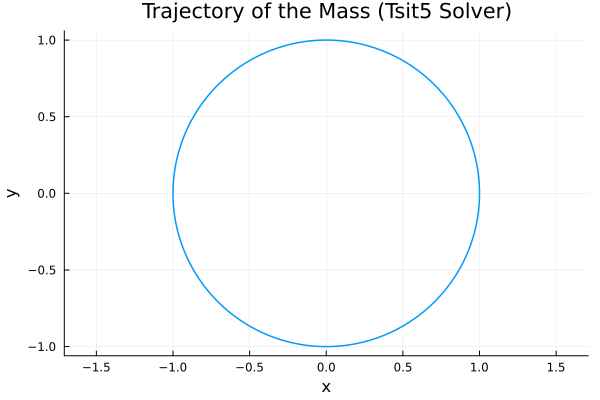
\includegraphics[width=0.5\linewidth]{Problems/Problem6/figures/circular_trajectory.png}
    \caption{Observed Circular Motion when $k = 1.0$, $m = 1.0$, $\vec{v}_0 = 1.0\; \hat{j}$ and $\vec{r} = 1.0 \; \hat{i}$}
    \label{fig:placeholder}
\end{figure}